\documentclass[12pt,a4paper]{article}

\usepackage[left=1in,top=1in,right=1in,bottom=1in]{geometry}
\usepackage[T1]{fontenc}
\usepackage[utf8]{inputenc}
\usepackage{minted}

\usepackage{courier}
\usepackage{indentfirst}
\usepackage{graphicx}
\usepackage[hidelinks]{hyperref}
\usepackage{tikz}
\usepackage{array}
\usepackage{tabularx}
\usepackage{enumitem}
\usepackage[ruled,vlined]{algorithm2e}
\SetAlFnt{\footnotesize}

\newcommand{\tab}[1]{\hspace*{25pt}}

\def\sectionskip{\medskip}
\def\sectionlineskip{\medskip}
\urlstyle{same}

\title{Title of Document}
\author{K. D. Sunera Avinash Chandrasiri (170081L)}

\begin{document}

% ======================================
% Cover Page
% ======================================

\begin{titlepage}
    \begin{tikzpicture}[overlay,remember picture]
    \end{tikzpicture}

    {\hfill\scshape\Large Final Report \par}
    {\hfill\scshape CS3242 Micro-controllers and Applications\par}
    {\vspace{.5cm}}
    {\hrule}
    \vspace{2.5cm}
    {\hfill\huge\bfseries Environment Monitoring IoT Device\par}
    {\hfill\huge\bfseries with Common Alert Protocol\par}
    \vspace{1cm}
    {\hfill\large K. D. Sunera Avinash Chandrasiri\par}
    {\hfill\large 170081L\par}
    \vfill
    \hfill \today \par
\end{titlepage}

\newpage


% ======================================
% Table of Contents
% ======================================

\tableofcontents
\newpage

% ======================================
% Scope of the project
% ======================================

\section{Introduction}

\subsection{Scope}

This project is a device developed using the
\textbf{NodeMCU 32S} micro-controller, which monitors
environment parameters such as \textbf{temperature,
    humidity, barometric pressure, and ambient
    light level}. The used micro-controller will
operate with low-power and via a wi-fi connection.
Even though the wi-fi connection network
availability may be unreliable, firmware
for the microcontroller is designed in a way
so that network unreliability would not
entirely hinder the operation of the sensor. \par

The device will connect with a remote server via
an HTTP request. Here the microcontroller will
use \textbf{CAP(Common Alert Protocol)} to deliver the
relevant parameters. This "server sync" will
happen once every 15 minutes. In these situations,
the device will send the mean and the standard
deviation of the samples the device collected
within that 15 minutes.  If the network connection
fails for some reason, the device would still cache
the requests(up to a certain extent) and resend/replay
those messages once the network reconnects. \par

The backend implemented for the project is a simple
server based off of python. It uses \textbf{flask}
framework and sqlite database. It simply accepts alert
notifications sent by the device and displays them
in a tabular manner. \par


\subsection{Features}

Following are some of the features available in the device.
Node that following list also includes the features that were
expected from the project as well as some special features.
\setlist{nolistsep}
\begin{itemize}[noitemsep]
    \item Measuring temperature, humidity, barometric pressure, and ambient light level.
    \item Syncing with the server every 15 minutes.
    \item Use Common Alert Protocol 1.2 to deliver the messages.
    \item Replay messages that failed to deliver to the server due to network issues.
    \item In case of replaying past messages, timestamp is also sent after retreiveing it via NTP, so the server can correctly order the messages.
    \item Create a unique session identifier at the initialization of the device.
    \item Support multi-device connections. Because of the above unique identifier, we can connect multiple devices to the server.
\end{itemize}

\newpage

\section{Design}

% ======================================
% Diagram to explain high-level design
% ======================================

\subsection{High Level Design}

Following the high level system diagram is shown.
The system will mainly consist of two major parts; embedded device and the remote server.
The device will use a Wi-Fi connection to connect to the remote server.

\begin{figure}[h]
    \centering
    \includegraphics[width=0.65\textwidth]{./images/high-level-1.png}
    \caption{High Level Deployment Diagram}
\end{figure}

The high-level diagram of the embedded device is shown below.
Here, the sensors required are connected; BMP180 (for pressure sensing),
DHT11 (for humidity and temperature sensing) and LDR(for light level sensing).

\begin{figure}[h]
    \centering
    \includegraphics[width=\textwidth]{./images/high-level-2.png}
    \caption{High Level Device Diagram}
\end{figure}

\noindent The device will run on 5V input voltage while the input/output high
voltage of the NodeMCU will be 3.3V.

\clearpage

\newpage

% ======================================
%  List of components and their cost
% ======================================

\subsection{Components and Cost Breakdown}


\begin{figure}[!htb]
    \minipage{0.25\textwidth}
    \centering
    \includegraphics[width=0.9\linewidth]{./images/nodemcu.jpg}
    \endminipage\hfill
    \minipage{0.25\textwidth}
    \centering
    \includegraphics[width=0.9\linewidth]{./images/bmp180.jpeg}
    \endminipage\hfill
    \minipage{0.25\textwidth}
    \centering
    \includegraphics[width=0.9\linewidth]{./images/dht11.jpg}
    \endminipage\hfill
    \minipage{0.25\textwidth}%
    \centering
    \includegraphics[width=0.9\linewidth]{./images/ldr.jpeg}
    \endminipage
    \caption{From left to right - NodeMCU, BMP180, DHT11, LDR}
\end{figure}


The Price Breakdown for the product components are given below.
The chosen micro-controller board was \textbf{NodeMCU ESP-32S IoT Dev Board}
mainly because of its inbuilt Wi-Fi capabilities and its specialization
on such tasks, especially on IoT field.
Apart form that, for the sensors, following sensors were chosen. \par

\begin{figure}[h]
    \begin{tabular}{lp{11.5cm}}
        \textbf{DHT11 Sensor}  & Temperature and Relative Humidity Sensor Module. Temperature range is 0°C to 50°C (±1°C) and Humidity Range is 20\% to 90\% (±1\%) Operating voltage is  3.5V to 5.5V. \\
        \textbf{BMP180 Sensor} & Barometric Pressure sensor module. Range is 300hPa to 1100 hPa with 0.02 hPa accuracy. Operating voltage is 1.8-6 V.                                                   \\
        \textbf{LDR}           & Light Dependent Resistor for measuring ambient light level.                                                                                                            \\
    \end{tabular}
    \label{fig:layers}
\end{figure}

\noindent Cost breakdown for the device excluding connectors, resistors, bread-boards, etc... is given below.

\vspace{3mm}

\noindent\begin{tabularx}{\linewidth}{|X|r|}
    \hline
    \bf Component Name                                          & \bf Subtotal (LKR) \\
    \hline
    \hline
    NodeMCU ESP-32S WiFi Bluetooth Dual Mode IoT Dev Board      & 1050.00            \\
    BMP180 Barometric Pressure, Temperature and Altitude Sensor & 185.00             \\
    DHT11 Temperature and Relative Humidity Sensor Module       & 250.00             \\
    LDR 4mm                                                     & 10.00              \\
    \hline
    \hline
    \bf  Total Amount (LKR)                                     & \bf 1495.00        \\
    \hline
\end{tabularx}

\vspace{3mm}

The cost could have been further reduced by using a \textbf{NodeMCU ESP-8266} board.
This costs about half of the NodeMCU ESP-32S price.
However, ESP-32S was cited as being more reliable than ESP-8266.
So, ESP-32S was used.

\newpage

% ======================================
% Schematic diagram giving all components
% ======================================

\subsection{Schematic Diagram}

\vspace{2cm}

\begin{figure}[h]
    \centering
    \includegraphics[width=0.95\textwidth]{./images/schematic.png}
    \caption{Schematic Diagram of the device}
\end{figure}

\begin{figure}[H]
    \centering
    \includegraphics[width=\textwidth]{./images/schematic_pcb.png}
    \caption{Schematic PCB view of the prototype}
\end{figure}

\newpage

% ======================================
% Description on how fault recovery options areimplemented
% ======================================

\section{Implementation}

\subsection{Fault Recovery Implementation}

A simple queuing mechanism was used to mitigate the issue of unstable connectivity.
The firmware would first add the CAP records to the queue and then, when sending the data,
all the content in the queue will be sent.
In case some packet sending failed, (either because of no connectivity or server not being available)
the response from the server would fail or have an error status code.
In this case, that CAP record would again be added to the queue.
The queue would contain a bound so as to stop all the old records from being
on the memory and leading to a risk of memory overflow. Because of this bound, and
the implementation of the queue, once the connectivity continues, the most recent
records will be sent out to  the server.

Apart from queueing messages, the NodeMCU ESP32S contains an independently controlled
WiFi module which connects to the network even when it is disconnected. So, the module
will reconnect to the network in the case it was disconnected from the server due to
some reason.

\subsection{Prototype Implementation}

\begin{figure}[H]
    \centering
    \includegraphics[width=0.9\textwidth]{./images/breadboard.png}
    \caption{Prototype Implementation Design - Breadboard View}
\end{figure}

\begin{minipage}{0.45\linewidth}
    \begin{figure}[H]
        \centering
        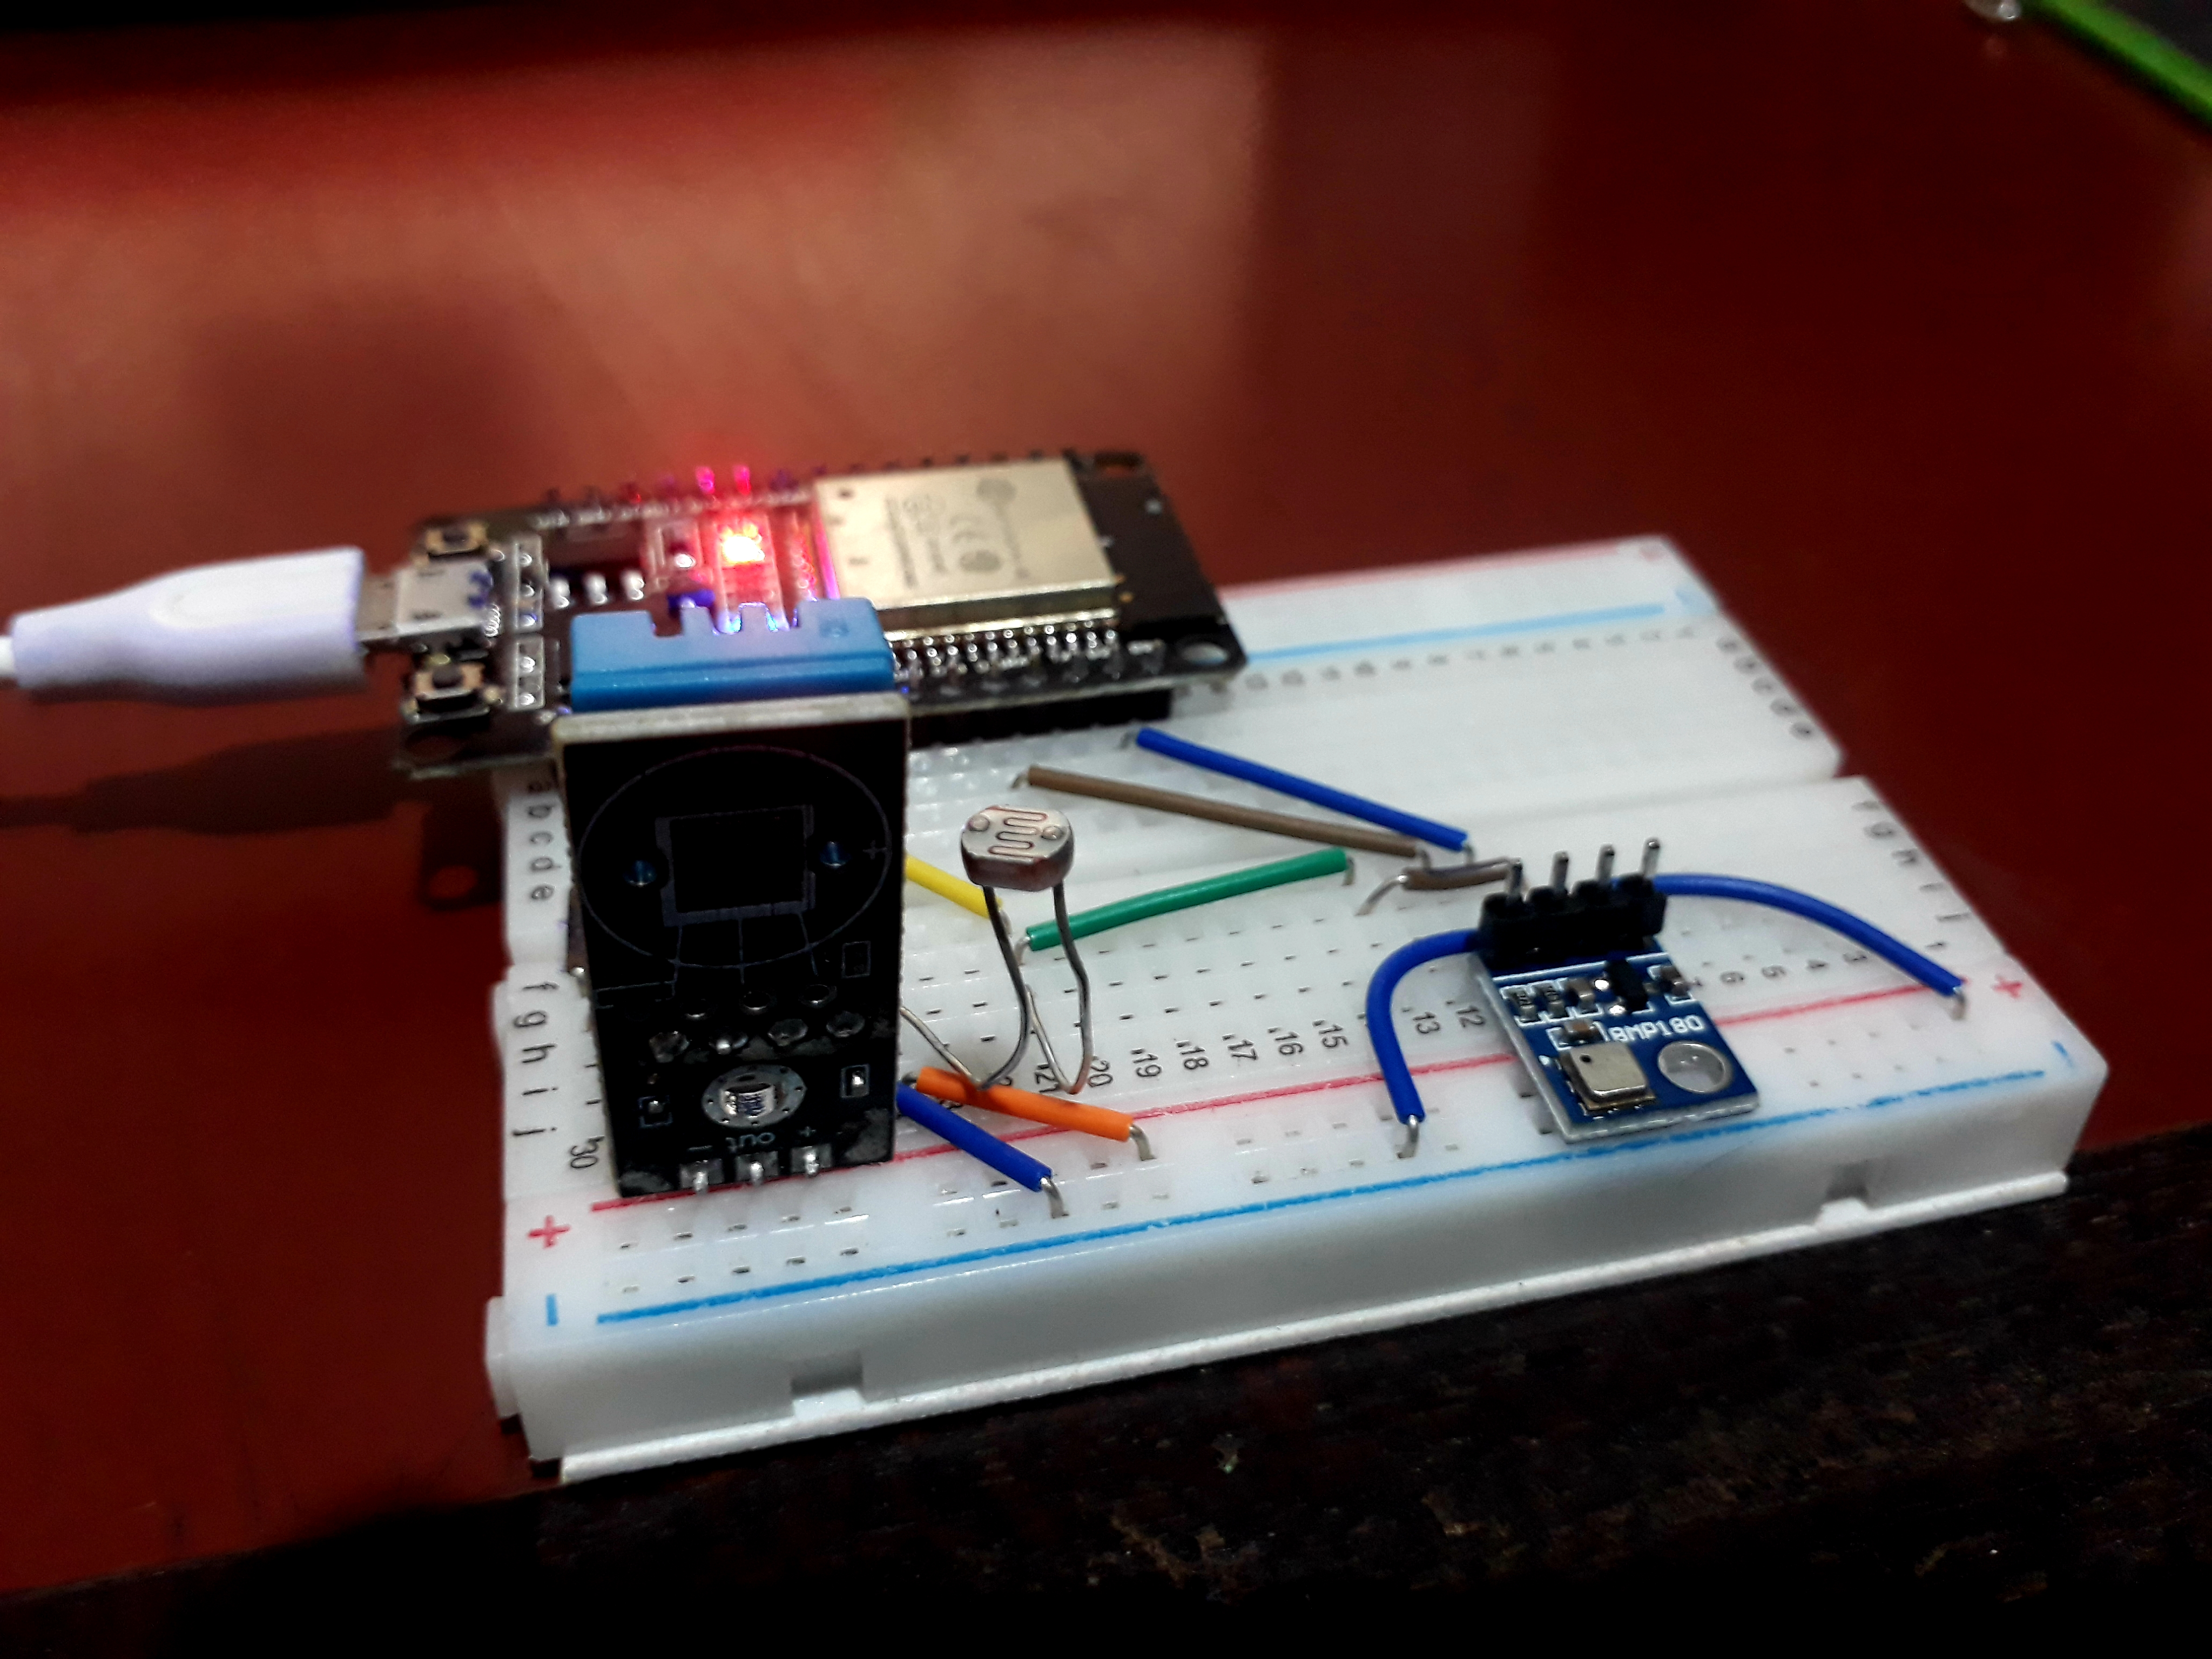
\includegraphics[width=\textwidth]{./images/device.jpg}
        \caption{Prototype Device}
    \end{figure}
\end{minipage}\hfil
\begin{minipage}{0.4\linewidth}
    As per the device implementation, I was able to connect the device as denoted in the
    above breadboard view and test it. However, due to some constraints  I was not able  to
    connect it to a dot-board or something similar.

    Furthermore, because of an issue with uploading to the microcontroller,
    I had to attach a capacitor to the EN pin. (Otherwise it would randomly fail)
\end{minipage}
\vspace{20pt}

As mentioned in the overview, the remote server part of the system was implemented using flask.
The database used for the prototype was a simple SQLite database.
Web interface of the prototype consisted of a simple table containing all the
sensor data that was received along with the timestamp that the data was recorded by the MCU.
Following is a screenshot of this web application dashboard.

\begin{figure}[H]
    \centering
    \includegraphics[width=0.9\textwidth]{./images/browser.png}
    \caption{Prototype Dashboard Screenshot}
\end{figure}

For the CAP implementation, CAP on the device side was done manually. (without any explicit libraries dedicated for CAP)
However, some caveats were used to send the required fields in the CAP XML request.

For the \textbf{timestamp field}, a NTP library was used. This would fetch the current time from a remote server.
For the \textbf{identifier field}, the device would first generate a random string of 32 characters.
This will be seeded by the voltage of 0 pin. (This is floating, thus ensuring randomness)
This 32-character string will be used as the session identifier.
Each message sent in this session would be suffixed by an incrementing integer.
This ensures that 2 devices can operate with the same server without any interference.

\newpage

% ======================================
% Algorithm used for device and server (Pseudo code)
% ======================================

\subsection{Algorithm}

\begin{algorithm}[H]
    \SetAlgoLined
    \SetKwInOut{Input}{input}\SetKwInOut{Output}{output}
    \DontPrintSemicolon
    \SetKwProg{Fn}{Function}{ is}{end}

    $queue \longleftarrow LifoQueue()$\;
    $tempSamples \longleftarrow array()$\;
    $humiditySamples \longleftarrow array()$\;
    $pressureSamples \longleftarrow array()$\;
    $lightSamples \longleftarrow array()$\;
    $samplesCollected \longleftarrow 0$\;
    \BlankLine

    \Fn{sendSamples()}{
        \tcp*{find mean \& std}
        $tempMean \longleftarrow mean(tempSamples)$\;
        \tcp{$...$}
        $lightStd \longleftarrow std(tempSlightSamplesamples)$\;
        \BlankLine
        \tcp*{Add message to end of queue}
        $cap \longleftarrow createCapMessage(tempMean, ..., lightStd)$\;

        \If {$queue.isFull()$}{
            $queue.pop()$\;
        }
        $queue.push(cap)$\;

        \BlankLine
        \tcp*{send all current messages}
        $currentQueueSize \longleftarrow queue.size()$\;
        \For{$i\leftarrow 0$ \KwTo $currentQueueSize$}{
            $capEntry \longleftarrow queue.pop()$\;
            $response \longleftarrow wifi.sendPostRequest(capEntry)$\;
            \tcp*{Re-add failed requests}
            \If {$response = ERR \lor response.status \neq 200$}{
                $queue.push(capEntry)$\;
            }
        }

        \BlankLine
        \tcp*{reset variables}
        $samplesCollected \leftarrow 0$\;
        $tempSamples.clear()$\;
        \tcp{$...$}
        $lightSamples.clear()$\;
    }


    \BlankLine
    \Fn{collectSamples()}{
        $temp \leftarrow readDHT11()$\;
        $humidity \leftarrow readDHT11()$\;
        $pressure \leftarrow readBMP180()$\;
        $light \leftarrow readLDR()$\;
        $tempSamples.add(temp)$\;
        \tcp{$...$}
        $lightSamples.add(light)$\;
        $samplesCollected++$\;
    }

    \BlankLine
    \Begin{
        \While{$True$}{
            \If {$timeSinceLastRead() \geq \Delta$}{
                \lIf{$samplesCollected == N$}
                { $sendSamples()$ }
                { $collectSamples()$ }
            }
        }
    }
    \caption{Pseudo code of the firmware}\label{algo}
\end{algorithm}\DecMargin{1em}
\clearpage

\newpage

% ======================================
% Full Source Code
% ======================================

\section{Annexure}

\definecolor{beige}{rgb}{0.96, 0.96, 0.86}
\definecolor{azure}{rgb}{0.94, 1.0, 1.0}

\newcommand{\PythonCode}[1]{\inputminted
    [fontsize=\footnotesize,frame=lines,framerule=1pt,
        label=REMOTE\_SERVER\StrGobbleLeft{#1}{10},framesep=10pt]
    {python}{#1}}
\newcommand{\HtmlCode}[1]{\inputminted
    [fontsize=\footnotesize,frame=lines,framerule=1pt,
        label=REMOTE\_SERVER\StrGobbleLeft{#1}{10},framesep=10pt]
    {html}{#1}}
\newcommand{\SqlCode}[1]{\inputminted
    [fontsize=\footnotesize,frame=lines,framerule=1pt,
        label=schema.sql,framesep=10pt]
    {sql}{#1}}
\newcommand{\CppCode}[1]{\inputminted
    [fontsize=\footnotesize,frame=lines,framerule=1pt,
        label=FIRMWARE\StrGobbleLeft{#1}{11},framesep=10pt]
    {c++}{#1}}



\subsection{Firmware Source Code}

\CppCode{../firmware/src/main.cpp}
\newpage
\CppCode{../firmware/src/utils.h}
\CppCode{../firmware/src/utils.cpp}
\newpage

\CppCode{../firmware/src/cap/cap.h}
\CppCode{../firmware/src/cap/statistic.h}
\CppCode{../firmware/src/cap/cap.cpp}
\newpage


\CppCode{../firmware/src/sensor/dht.h}
\CppCode{../firmware/src/sensor/dht.cpp}
\newpage
\CppCode{../firmware/src/sensor/bmp180.h}
\CppCode{../firmware/src/sensor/bmp180.cpp}
\CppCode{../firmware/src/sensor/ldr.h}
\CppCode{../firmware/src/sensor/ldr.cpp}
\newpage
\CppCode{../firmware/src/sensor/sensor.h}
\CppCode{../firmware/src/sensor/sensor.cpp}
\newpage

\CppCode{../firmware/src/wifi/config.h}
\CppCode{../firmware/src/wifi/controller.h}
\CppCode{../firmware/src/wifi/ntp.h}
\newpage
\CppCode{../firmware/src/wifi/controller.cpp}
\CppCode{../firmware/src/wifi/ntp.cpp}
\newpage


\subsection{Remote Server Source Code}

\PythonCode{../backend/app.py}
\newpage
\PythonCode{../backend/db/entry.py}
\newpage
\PythonCode{../backend/db/database.py}
\newpage
\HtmlCode{../backend/templates/index.html}
\newpage

\subsection{Remote Server Database Schema}

\SqlCode{../backend/db/schema.sql}
\newpage

% ======================================
% References
% ======================================

% \begin{thebibliography}{9}

%     \bibitem{bib:fritzing}
%     \url{https://fritzing.org/} - Fritzing tool was used to design the schematic diagrams of the prototype.


% \end{thebibliography}

\end{document}

